\chapter{Primer}
\section{Coordinate System Type}
We use the right handed coordinate system similar to the OpenGL coordinate system through out this project. To visualize this, make the first three fingers of your right hand mutually perpendicular. The thumb is the +z axis, index finger is the +x axis and middle finger is the +y axis. If you align this to a computer display, you can infer that to move an object (e.g. camera) inwards, you have to decrease the z value.
\begin{figure}[htbp]
    \centering
    % --- Right-handed 3D coordinate system ---
    \begin{subfigure}[b]{0.45\textwidth}
        \centering
        \begin{tikzpicture}[line cap=round,line join=round,>=stealth,scale=1.5]
            \draw[->, thick] (0,0,0) -- (1.2,0,0) node[anchor=north east] {$+X$};
            \draw[->, thick] (0,0,0) -- (0,1.2,0) node[anchor=south west] {$+Y$};
            \draw[->, thick] (0,0,0) -- (0,0,1.2) node[pos=1, anchor=south, xshift=-6pt] {$+Z$};
	  \end{tikzpicture}
        \caption{Right Handed Coordinate System}
    \end{subfigure}
    \hfill
    % --- 2D coordinate system ---
    \begin{subfigure}[b]{0.45\textwidth}
        \centering
        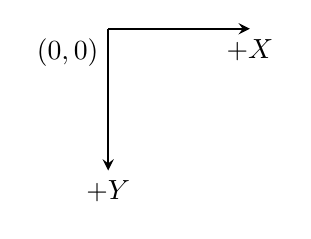
\begin{tikzpicture}[>=stealth,scale=1.5]
            \draw[->, thick] (0,0) -- (1.2,0) node[anchor=north] {$+X$};
            \draw[->, thick] (0,0) -- (0,-1.2) node[anchor=north] {$+Y$};
            \node at (0,0) [anchor=north east] {$(0, 0)$};
        \end{tikzpicture}
        \caption{2D coordinate system}
    \end{subfigure}
    \caption{Coordinate systems used throughout this project.}
\end{figure}

The 2D framework we use has x coordinates increasing from left to right and y coordinates increasing from top to bottom.
\section{3D Model}
In our engine, each 3D model is a list of triangles, each triangle is list of three vertices and each vertex has three attributes. Those attributes are position, normal and texture coordinate. 
\subsection{Example of our simple object file}
We use Wavefront Object format for storing this information as a text file. The following is such a file for a cube. Note that, in a line, anything after \# is a comment. 
\lstset{style=general}
\begin{lstlisting}
v 1 1 -1			#top-right point in back face : v1
v 1 -1 -1			#bottom-right point in back face: v2
v 1 1 1			#top-right point in front face: v3
v 1 -1 1			#bottom-right point in front face: v4
v -1 1 -1			#top-left point in back face: v5
v -1 -1 -1		#bottom-left point in in back face: v6
v -1 1 1			#top-left point in front face: v7
v -1 -1 1			#bottom-left point in front face: v8
vn 0 1 0			#up : vn1
vn 0 0 1			#front: vn2
vn -1 0 0			#left: vn3
vn 0 -1 0			#down: vn4
vn 1 0 0			#right: vn5
vn 0 0 -1			#back: vn6
vt 0 1				#top-left: vt1
vt 1 0				#bottom-right: vt2
vt 1 1				#top-right: vt3
vt 0 0				#bottom-left: vt4
f 5/1/1 3/2/1 1/3/1 #(v5, vt1, vn1), (v3, vt2, vn1), (v1, vt3, vn1)
f 3/3/2 8/4/2 4/2/2 #(v3, vt3, vn2), (v8, vt4, vn2), (v4, vt2, vn2)
f 7/1/3 6/2/3 8/4/3 #(v7, vt1, vn3), (v6, vt2, vn3), (v8, vt4, vn3)
f 2/3/4 8/4/4 6/1/4 #(v2, vt3, vn4), (v8, vt4, vn4), (v6, vt1, vn4)
f 1/3/5 4/4/5 2/2/5 #(v1, vt3, vn5), (v4, vt4, vn5), (v2, vt2, vn5)
f 5/1/6 2/2/6 6/4/6 #(v5, vt1, vn6), (v2, vt2, vn6), (v6, vt4, vn6)
f 5/1/1 7/4/1 3/2/1 #(v5, vt1, vn1), (v7, vt4, vn1), (v3, vt2, vn1)
f 3/3/2 7/1/2 8/4/2 #(v3, vt3, vn2), (v7, vt1, vn2), (v8, vt4, vn2)
f 7/1/3 5/3/3 6/2/3 #(v7, vt1, vn3), (v5, vt3, vn3), (v6, vt2, vn3)
f 2/3/4 4/2/4 8/4/4 #(v2, vt3, vn4), (v4, vt2, vn4), (v8, vt4, vn4)
f 1/3/5 3/1/5 4/4/5 #(v1, vt3, vn5), (v3, vt1, vn5), (v4, vt4, vn5)
f 5/1/6 1/3/6 2/2/6 #(v5, vt1, vn6), (v1, vt3, vn6), (v2, vt2, vn6)

\end{lstlisting}
\subsection{Vertex Attribute 1: Positions}
Vertex positions contain the object space (x, y, z) co-ordinates in floating point format. Object space is the coordinate system defined by the model designer when creating the model.\\An example for a vertex position line in the file is "v 1 1 -1". Note that it starts with `v'. Since a cube has 8 corners, we can see eight position-lines in the file.
\subsection{Vertex Attribute 2: Normals}
We need normals for lighting calculations.
If we take the cross product of adjacent edges of vertex in a triangle we get the face normal of the
triangle. A vertex can be common to many triangles. The vertex normal is the normalized average vector
of the face normals of such triangles. Or it can be just the face normal. \\An example of a vertex normal line in the file is "vn 0 1 0". Note that it stars with `vn'.  Since a cube has 6 faces, we can see six normal-lines in the file.
\subsection{Vertex Attribute 3: Texture Coordinates}
Textures add convincing visual quality to the model. Texture coordinates contain the UV mapping information. Each texture coordinate corresponds to the  location of the image used by the vertex for mapping texture. If we know the three texture coordinates that corresponds to three vertices we can find the texture coordinate for any point on the triangle formed by the three vertices.\\An example of texture coordinate line in the file is "vt 0 1". Note that it stars with `vt'. Here an image is mapped to each face of the cube. So we can see four corners of the image as texture-coordinate-lines.
\subsection{Triangles}
A triangle definition contain three vertex attribute index set that correspond to each of the three vertices.\\A triangle line starts with `f' which stands for face. There is another Wavefront object file format in which the face line has definition for quadrilateral. \\Lets interpret the following triangle line in the file: \\
"f 5/1/1 3/2/1 1/3/1" \\
Interpretation:\\
The attributes of the first vertex:\\
Position: 5th  vertex postion listed: v -1 1 -1 \\
Texture coordinate: 1st texture coordinate listed: vt 0 1\\
Normal: 1st normal listed: vn 0 1 0\\

The attributes of the second vertex:\\
Position: 3rd  vertex postion listed: v 1 1 1\\
Texture coordinate: 2nd texture coordinate listed: vt 0 1\\
Normal: 1st normal listed:vn 0 1 0\\

The attributes of the third  vertex:\\
Position: 1st  vertex postion listed: v 1 1 -1\\
Texture coordinate: 3rd texture coordinate listed: vt 1 0\\
Normal: 1st normal listed: vn 0 1 0\\

\section{Translation}
The action causing linear displacement of a point is called translation. Let $A$ be the initial point and $B$ be the translated point. The translation vector can be defined as:

\begin{align*}
\vec{t} &= B - A
\end{align*}

This can be rearranged to express the translated point in terms of the initial point and the translation vector:

\begin{align*}
B &= A + \vec{t}
\end{align*}

Let  $A$ be the point \( (x, y, z) \) and $B$ be the point \( (x', y', z') \) and $\vec{t}$ be the vector \( (t_x, t_y, t_z) \). Then
\begin{equation}
\begin{aligned}
x' &= x + t_x \\
y' &= y + t_y \\
z' &= z + t_z
\end{aligned}
\end{equation}

\section{Scaling}
The expansion or shrinking of a point's distance from the origin is known as scaling with respect to origin. The scaling can make objects bigger or smaller in size. 

Let $s_x$, $s_y$, $s_z$ be the scaling factors. Then the scaling is defined as follows.
\[
\begin{aligned}
x' &= x \cdot s_x \\
y' &= y \cdot s_y \\
z' &= z \cdot s_z
\end{aligned}
\]
The vector equation for scaling is the Hadamard product of original vector $P$ and scaling vector $S$.
\[
P = P \circ  S
\]

\section{Rotation}
The action that causes an angular displacement of a point around an axis is called rotation. Since rotation is the circular motion of a point by a certain angle, we need to calculate the sine and cosine of that angle and do some calculations with the original point to get the resultant point. 

Consider a point \(P(x, y, 0)\), at a distance \(r\) from the origin \(O\).

Suppose that the line \(OP\) makes the angle \(\theta\) with the \(x\)-axis. 
Then 
\begin{equation}
\begin{aligned}
x = r \cdot \cos \theta \\
y =  r \cdot \sin \theta
\end{aligned}    
\label{eq:param_circle}
\end{equation}

\begin{minipage}[t]{0.7\textwidth}
Suppose now that we rotate \(P\) counterclockwise by an angle \(\phi\) with respect to the line \(OP\) to obtain the point \(Q\). Let \((x', y', 0)\) define \(Q\). Then:

\[
x' = r \cdot \cos (\theta + \phi)
\]
\[
y' = r \cdot \sin (\theta + \phi)
\]
\end{minipage}%
\hfill
\begin{minipage}[t]{0.28\textwidth}

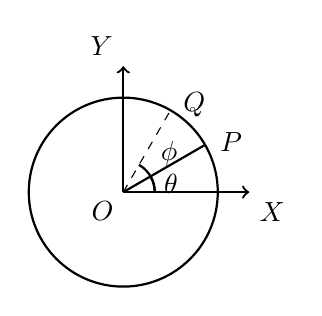
\begin{tikzpicture}[scale=0.8]
\draw[thick, ->] (0,0) -- (2,0) node[anchor=north west] {$X$};
\draw[thick, ->] (0,0) -- (0,2) node[anchor=south east] {$Y$};
\draw[thick] circle (1.5);
\node[anchor=north east] at (0,0) {$O$};

\draw[thick] (0,0) -- (30:1.5); 
\draw[dashed] (0,0) -- (60:1.5);    

\node[anchor=west] at (30:1.6) {$P$};
\node[anchor=west] at (60:1.6) {$Q$};

\draw[thick] (0.5,0) arc[start angle=0, end angle=30, radius=0.5] node[midway, right] {$\theta$};

\draw[thick] (0.5,0) arc[start angle=0, end angle=60, radius=0.5] node[midway, above right] {$\phi$};

\end{tikzpicture}


\end{minipage}


Expanding \(x'\) using the trigonometric identity for \(\cos(A+B)\):
\[
x' = r \cdot [\cos \theta \cos \phi - \sin \theta \sin \phi]
\]
\[
x' = r \cdot \cos \theta \cos \phi - r \cdot \sin \theta \sin \phi
\]
From equations ~\eqref{eq:param_circle},
\begin{equation}
    x' = x \cdot \cos \phi - y \cdot \sin \phi
\end{equation}
Similarly, we can derive the expression for \(y'\) using \(\sin(A+B)\) 
\begin{equation}
y' = x \cdot \sin \phi + y \cdot \cos \phi.
\end{equation}
That derivation is left as an exercise for the reader.


\section{Homogeneous Representation}
Homogeneous representation is a technique used to unify transformations, such as translation, rotation, scaling, and projection. Points and vectors are given an extra coordinate, denoted as $w$. The $w$ component of points will be 1, while that of vectors will be 0. Instead of $3 \times 3$ matrices, the transformations are represented using $4 \times 4$ matrices, which can be multiplied together. From now on, we use homogeneous representation to represent transformations.
\section{Derivation of Translation Matrix}
A translation transformation is like a black box with an input and an output. The processing element is the translation matrix. For translation, we already know the input and output. Our translation matrix should be a homogeneous matrix of the order $4\times4$. Therefore, we should specify input and output in homogeneous coordinates. Let a point \(A(x, y, z, 1)\) be translated to the point \(B(x+t_x, y+t_y, z+t_z, 1)\) by the translation matrix \(T\).
The transformation equation is: \[T \cdot A = B \]

Or:
\[
\begin{bmatrix}
a_{00} & a_{01} & a_{02} & a_{03} \\
a_{10} & a_{11} & a_{12} & a_{13} \\
a_{20} & a_{21} & a_{22} & a_{23} \\
a_{30} & a_{31} & a_{32} & a_{33}
\end{bmatrix}
\cdot
\begin{bmatrix}
x \\
y \\
z \\
1
\end{bmatrix}
=
\begin{bmatrix}
x + t_x \\
y + t_y \\
z + t_z \\
1
\end{bmatrix}
\]
Expanding the LHS we get,
\[
\begin{bmatrix}
a_{00} \cdot x & a_{01} \cdot y  & a_{02} \cdot z  & a_{03} \cdot 1 \\
a_{10} \cdot x  & a_{11} \cdot y  & a_{12} \cdot z  & a_{13} \cdot 1 \\
a_{20} \cdot x  & a_{21} \cdot y  & a_{22} \cdot z  & a_{23} \cdot 1 \\
a_{30} \cdot x  & a_{31} \cdot y  & a_{32} \cdot z  & a_{33} \cdot 1  
\end{bmatrix}
=
\begin{bmatrix}
x + t_x \\
y + t_y \\
z + t_z \\
1
\end{bmatrix}
\]
Equating the  first rows in both LHS and RHS, we get:
\begin{align*}
a_{00} \cdot x &+ a_{01} \cdot y + a_{02} \cdot z + a_{03} \cdot 1 = x + t_x
\end{align*}
We can deduce that $a_{00} = 1, a_{01} = 0,a_{02} = 0,a_{03} = t_x$\\
By making similar deductions for all rows, we can calculate all elements of the matrix \(T\).
\begin{equation}
T =
\begin{bmatrix}
1 & 0  & 0  & t_x \\
0 & 1  & 0  & t_y \\
0 & 0  & 1  & t_z \\
0 & 0  & 0  & 1 \\
\end{bmatrix}
\end{equation}
\section{Derivation of Scaling Matrix}
Let a point \(A(x, y, z, 1)\) be scaled to the point \(B(x \cdot s_x, y \cdot s_y, z \cdot s_z, 1)\) by the scaling matrix \(S\).
The scaling transformation equation is: \[S \cdot A = B \]
Or:
\[
\begin{bmatrix}
a_{00} & a_{01} & a_{02} & a_{03} \\
a_{10} & a_{11} & a_{12} & a_{13} \\
a_{20} & a_{21} & a_{22} & a_{23} \\
a_{30} & a_{31} & a_{32} & a_{33}
\end{bmatrix}
\cdot
\begin{bmatrix}
x \\
y \\
z \\
1
\end{bmatrix}
=
\begin{bmatrix}
x \cdot s_x \\
y \cdot s_y \\
z  \cdot s_z \\
1
\end{bmatrix}
\]
By the deduction technique we used in the previous section, we can find the required matrix as follows.
\begin{equation}
S =
\begin{bmatrix}
s_x & 0  & 0  & 0 \\
0 & s_y  & 0  & 0 \\
0 & 0  & s_z  & 0 \\
0 & 0  & 0     & 1 \\
\end{bmatrix}
\end{equation}

\section{Derivation of Rotation Matrix}
We are deriving the rotation matrix which will rotate any point around \(Z-axis\). We already know the expression for rotating any point about the origin in the \(XY\) plane, i.e., when \(z=0\). The expressions are 

\[
 x' = x \cdot \cos \phi - y \cdot \sin \phi 
\]
\[
y' = x \cdot \sin \phi + y \cdot \cos \phi
\]

If we never change the z coordinate during rotation, we will get the required rotation. For that purpose, we just have to add the following.
 \[
 z' = z
 \]
A rotation transformation is also a black box with an input, a rotation matrix (processing element), and an output. Let the input and output as points be \(A(x, y, z, 1)\) and \(B(x', y', z', 1)\) and the rotation matrix be \(R_z\).
The transformation equation is \[R_z \cdot A = B \]

Or:
\[
\begin{bmatrix}
r_{00} & r_{01} & r_{02} & r_{03} \\
r_{10} & r_{11} & r_{12} & r_{13} \\
r_{20} & r_{21} & r_{22} & r_{23} \\
r_{30} & r_{31} & r_{32} & r_{33}
\end{bmatrix}
\cdot
\begin{bmatrix}
x \\
y \\
z \\
1
\end{bmatrix}
=
\begin{bmatrix}
x' \\
y' \\
z'  \\
1
\end{bmatrix}
\]
Expanding the LHS and RHS we get,
\[
\begin{bmatrix}
r_{00} \cdot x & r_{01} \cdot y  & r_{02} \cdot z  & r_{03} \cdot 1 \\
r_{10} \cdot x  & r_{11} \cdot y  & r_{12} \cdot z  & r_{13} \cdot 1 \\
r_{20} \cdot x  & r_{21} \cdot y  & r_{22} \cdot z  & r_{23} \cdot 1 \\
r_{30} \cdot x  & r_{31} \cdot y  & r_{32} \cdot z  & r_{33}\cdot 1  
\end{bmatrix}
=
\begin{bmatrix}
 x \cdot \cos \phi - y \cdot \sin \phi \\
x \cdot \sin \phi + y \cdot \cos \phi \\
z  \\
1
\end{bmatrix}
\]
Equating the  first and second rows in both LHS and RHS, we get:
\begin{align*}
r_{00} \cdot x &+ r_{01} \cdot y + r_{02} \cdot z + r_{03} \cdot 1 = x \cdot \cos \phi - y \cdot \sin \phi \\
r_{10} \cdot x &+ r_{11} \cdot y + r_{12} \cdot z + r_{13} \cdot 1 = x \cdot \sin \phi + y \cdot \cos \phi
\end{align*}
We can deduce that \\ $r_{00} = \cos \phi, r_{01} = -\sin \phi,r_{02} = 0,r_{03} = 0$\\ $r_{10} = \sin \phi, r_{11} = \cos \phi, r_{12} = 0, r_{13} = 0$\\
By making similar deductions for all rows, we can calculate all elements of the matrix \(R_z\).
\begin{equation}
R_z =
\begin{bmatrix}
\cos \phi & -\sin \phi & 0 & 0 \\
\sin \phi & \cos \phi  & 0 & 0 \\
0         & 0          & 1 & 0 \\
0         & 0          & 0 & 1
\end{bmatrix}
\end{equation}

Similarly you can derive \(R_x\) and \(R_y\). That is left as an excersise.
\section{Modeling Transformations}
The transformations scaling, rotation and translations are the main modeling transformations. They are used to place a 3D object in the correct scale, orientation and position at the world coordinate system defined in the rendering application. They are applied in the following order.
\begin{equation}
M = T \cdot R \cdot S
\end{equation}
Where $T$, $R$, and $S$ are matrices for translation, rotation and scaling transformations.  $R$ it self can be composed of $x$, $y$, and $z$ rotations. We follow the following composition of rotations.
\begin{equation}
R = R_z \cdot R_x \cdot R_y
\end{equation}

\section{Linear Interpolation}
Linear Interpolation is the calculation of in-between values in a range of numbers. For example, if we want the in-between value $x$ in the range from 24 to 78 with an interpolation factor of 0.3, then:

\[
x = 24 + (78 - 24) \cdot 0.3 = 40.2
\]

Also,

\[
x = 24 \cdot (1 - 0.3) + 78 \cdot 0.3
\]

which simplifies to:

\[
x = 24 \cdot 0.7 + 78 \cdot 0.3
\]

In general, linear interpolation can be expressed as:

\begin{equation}
x = a + (b - a) \cdot f
\end{equation}

where $a$ is the initial value, $b$ is the final value, and $f$ is the interpolation factor.


\subsection {Speeding up Linear Interpolation}
Consider the case of interpolating from one intensity value to another along a scanline. We can find the intensity at any point can be calculated by the following formula.
\[ 
I_x = I_1 + \frac{(I_2 - I_1)}{(x_2 - x_1)}  \cdot {(x-x_1)}
\]
But remember we increment $x$ by $1$ to do the calculations because we are dealing with pixel array for a screen.
There is a faster alternative than to apply the above formula for every such $x$ along the endpoints $x_1$ and $x_2$. ie., we can precalculate intensity increment by the following formula for each unit increment of $x$ and accumulate intensity at each step to get the intensity for $x$.

\[ 
\Delta I = \frac{(I_2 - I_1)}{(x_2 - x_1)}
\]

Initially:
\[ 
I_x \leftarrow I_1
\]

At each unit increment of x:
\[ 
I_x \leftarrow I_x + \Delta I
\]
\subsection{Interpolation using Signed Distances}
Consider two values on the 1D  real number line.
\begin{align*}
A &= 10\\
B &= 40
\end{align*}

Let P be an in-between value.
\begin{align*}
P &= 15
\end{align*}

\begin{center}
\begin{tikzpicture}[scale=0.2]
  % Axis
  \draw[<->] (0,0) -- (50,0) node[below right] {};

  % Points
\draw[fill=black] (10,0) circle (0.2) node[above] {A};
\draw[dashed, gray] (10,0) -- (10,-8);
\node at (10,-10) {10};

\draw[fill=black] (15,0) circle (0.2) node[above] {P};
\draw[dashed, gray] (15,0) -- (15,-8);
\node at (15,-10) {15};

\draw[fill=black] (40,0) circle (0.2) node[above] {B};
\draw[dashed, gray] (40,0) -- (40,-8);
\node at (40,-10) {40};
  % Arrows for distances
  \draw[->, thick,] (15,-3) -- (10,-3) node[midway, below] {\(d1\)};
  \draw[->, thick] (15,-5) -- (40,-5) node[midway, below] {\(d2\)};
\end{tikzpicture}
\end{center}

Then the signed distances to A and B from P are:
\begin{align*}
d1 &= PA = A - P = 10 - 15 = -5\\
d2 &= PB = B - P = 40 - 15 = 25
\end{align*}

The signed distance ratio is
\begin{align*}
t &=  \frac{d1}{d1-d2} =  \frac{-5}{-5-25} = \frac{1}{6} \\
\end{align*}

That $t$ is the interpolation factor.
i.e.,
\[
15 = 10 \cdot (1 - \frac{1}{6}) + 40 \cdot \frac{1}{6}\\
\]


\section{Barycentric Interpolation}
We use barycentric interpolation to estimate vertex attributes for a point inside a triangle.  
The vertex attributes can include texture coordinates, colors,  depth, and more.
First, the barycentric coordinates for a candidate pixel --- denoted by $\alpha$, $\beta$, and $\gamma$ --- are calculated such that:
\[
\alpha + \beta + \gamma = 1
\]
Once $\alpha$, $\beta$, and $\gamma$ are known, the estimated vertex attribute at the candidate pixel $P$ is calculated using:

\begin{equation}
Attib_P = \alpha \cdot Attrib_A + \beta \cdot Attrib_B + \gamma \cdot Attrib_C
\end{equation}


\section{Camera}
The camera is like a tiny window through we which see the virtual world. 
The modification of the camera parameters viz., eye, target, look direction, field of view angle, near plane distance, far plane distance etc., affects the view matrix and projection matrix calculations. This will cause the renderer to render different parts of the scene. When done interactively based on user input, it creates an experience of exploring  the virtual world.
\subsection{Viewing}
The camera has a position in world space and it has local axes and Euler angles\footnote{Euler angles are the three rotations about the mutually perpendicular local axes. They are called yaw, pitch and roll} for representing the camera orientation. The camera direction is determined by the camera target point. \footnote{The camera is in a right handed coordinate system, we see the world from the negative axis of the camera. Therefore we calculate the target to eye vector and use it for calculating the $+z$ axis of the camera.} The camera can be translated and or rotated.  When we apply the translation we apply the same amount of translation to both the camera position and the target point and the view matrix is recalculated. To rotate the camera, we modify the euler angles and then the view matrix is recalculated from euler angles. Another way to rotate the target point and recalculate the view matrix.

Given the camera position $E$ (also called `eye'), the target point $T$ (also called `at'), and the camera up vector $U$, we compute the view matrix as follows: \\
N.B.: All points are world space coordinates.\\

\begin{equation}
\begin{aligned}
\text{Back vector:}\quad \vec{b} &= E - T \\
\text{Normalized Back vector:}\quad \hat{b} &= \frac{\vec{b}}{\|b\|} \\
\text{Normalized Up vector:}\quad \hat{U} &= \frac{\vec{U}}{\|U\|} \\
\text{Right vector:}\quad \vec{r} &= \hat{U} \times \hat{b} \\
\text{Normalized Right vector:}\quad  \hat{r} &= \frac{\vec{r}}{\|r\|} \\
\text{True up vector:}\quad \vec{t} &= \hat{b} \times \hat{r}\\
\text{Normalized True up vector:}\quad  \hat{t} &= \frac{\vec{t}}{\|t\|} 
\end{aligned}
\end{equation}

The view matrix $V$ is formed by placing the normalized basis vectors\footnote{Normalized Back Vector, Normalized Right Vector and Normalized True Up Vector} and the translation terms into a $4\times 4$ matrix:
\begin{align*}
V =
\begin{pmatrix}
\hat{r}_x & \hat{r}_y & \hat{r}_z & -\,\hat{r}\;\cdot\;E \\
\hat{t}_x & \hat{t}_y & \hat{t}_z & -\,\hat{t}\;\cdot\;E \\
\hat{b}_x & \hat{b}_y & \hat{b}_z & -\,\hat{b}\;\cdot\;E\\
0         & 0         & 0         & 1
\end{pmatrix}.
\end{align*}
\begin{equation}
V =
\begin{pmatrix}
\hat{r}_x & \hat{r}_y & \hat{r}_z & -\,E_x \\
\hat{t}_x & \hat{t}_y & \hat{t}_z & -\,E_y \\
\hat{b}_x & \hat{b}_y & \hat{b}_z & -\,E_z\\
0         & 0         & 0         & 1
\end{pmatrix}.
\end{equation}
The above matrix is obtained by the concatenation of rotation matrix and translation matrix. 

The translation part is needed because we need to shift the world space origin to camera location and the rotation is needed because we need to align the world space axes to camera space axes. That special type of rotation is a topic in Linear Algebra and called change of basis. The interested readers can research on that topic for why our rotation part of view matrix is formed with the camera axes like the following.

View matrix rotation part is:
\begin{equation}
R =
\begin{pmatrix}
\hat{r}_x & \hat{r}_y & \hat{r}_z & 0 \\
\hat{t}_x & \hat{t}_y & \hat{t}_z & 0 \\
\hat{b}_x & \hat{b}_y & \hat{b}_z & 0 \\
0         & 0         & 0         & 1
\end{pmatrix}
\end{equation}

View matrix translation part is:
\begin{equation}
T =
\begin{pmatrix}
1 & 0 & 0 & -\,E_x \\
0 & 1 & 0 & -\,E_y \\
0 & 0 & 1 & -\,E_z  \\
0 & 0 & 0 & 1
\end{pmatrix}
\end{equation}

It can be verified that $V = R \cdot T$


\subsection{Orthographic Transform}
The Orthographic projection is used to render objects in their true size. This is useful for 2D games and CAD.
Here we will see how the projection matrix is calculated using this method.\\
In the orthographic projection, the lengths are preserved, but we have to remap the coordinates as follows.
The orthographic projection matrix is derived from the six camera view bounds that we specify. They are left, right, bottom, top, near, and far. We will refer to this bound as $(l, r, b, t, n, f)$ further in this chapter. The coordinate component of any point $(x, y,$ or $z)$ in the camera space has to be transformed in the range $-1$ to $+1$. We need that step because that makes clipping easy.

First we will derive a general equation, that will convert any interval $[a,b]$ to $[-1,+1]$\\
Let $\kappa$ be any value inside $[a,b]$ and $\lambda$ be the corresponding mapped value inside $[-1,+1]$\\
\begin{align*}
\text{Then,}\quad \frac{\kappa-a}{b-a} = \frac{\lambda+1}{2}
\end{align*}

\begin{equation}
\text{Or,}\quad \lambda = \frac{2 \cdot (\kappa-a)}{b-a} - 1
\label{eq:normalize_value}
\end{equation}



Now we can map $x$ inside $[l,r]$ to $x'$ inside $[-1, +1]$, by using~\eqref{eq:normalize_value}.
by sustituting the following values.
\begin{align*}
&\lambda = x' \\
&\kappa = x \\
&a = l \\
&b = r
\end{align*}
And the mapping is
\begin{align*}
x' &= \frac{2 \cdot (x - l)}{r - l} - 1 
\end{align*}
By algebraic manipulation we arrive at the following version of it,
\begin{equation}
  x' = \frac{2 \cdot x}{r-l} - \frac{r+l}{r-l}
\end{equation}
Similarly, for $y$ we get the following.
\begin{equation}
  y' = \frac{2 \cdot y}{t-b} - \frac{t+b}{t-b}
\end{equation}
For $z$, we have to negate it first.\footnote{It is so because,our coordinate system is right handed and what we see is the $-z$ axis portion of the camera view axes. Recall that from the coordinates of the world space \texttt{eye} and \texttt{at} , we calculate the view axis $z$ (which we denote as $n$) from the vector: $\texttt{eye} - \texttt{at}$. So we get $z$ coordinates as negative values. If they need to satisfy the inequality $n \leq \texttt{zvalue} \leq f$, they need to be negated.}

\begin{equation}
  z' = \frac{-2 \cdot z}{f-n} - \frac{f+n}{f-n}
\end{equation}


We can arrive at the following inequality for z.

\begin{align}
  -1 \leq \frac{-2 \cdot z}{f-n} - \frac{f+n}{f-n} \leq +1
\end{align}

Using the results we obtained so far in this section, we can write the orthographic equation as:
\[
\begin{bmatrix}
a_{00} & a_{01} & a_{02} & a_{03} \\
a_{10} & a_{11} & a_{12} & a_{13} \\
a_{20} & a_{21} & a_{22} & a_{23} \\
a_{30} & a_{31} & a_{32} & a_{33}
\end{bmatrix}
\cdot
\begin{bmatrix}
x \\
y \\
z \\
1
\end{bmatrix}
=
\begin{bmatrix}
\frac{2 \cdot x}{r-l} - \frac{r+l}{r-l}\\
\frac{2 \cdot y}{t-b} - \frac{t+b}{t-b}\\
\frac{-2 \cdot z}{f-n} - \frac{f+n}{f-n}\\
1
\end{bmatrix}
\]

By the deduction technique used in the previous sections, we can find the required matrix as:
\begin{equation}
\begin{bmatrix}
\frac{2}{r-l} & 0 & 0 &-\frac{r+l}{r-l} \\
0 & \frac{2}{t-b} & 0 &-\frac{t+b}{t-b} \\
0 & 0 & \frac{-2}{f-n} & -\frac{f+n}{f-n} \\
0 & 0 & 0 & 1
\end{bmatrix}
\end{equation}
By analyzing the result we got, we can see that the orthographic projection transformation is a composite of the following transforms.
\vspace{1em}
\begin{enumerate}
    \item Translation that shifts the center of the view volume to the origin
    \item Scale that scales the view volume to the canonical viewing volume size
\end{enumerate}
\vspace{1em} 
\subsection{Perspective Transform}
Perspective projection is the method used by the rendering engines to make near objects appear big and distant objects appear small. The effect is called perspective foreshortening. The goal of the perspective transform and the subsequent perspective divide operation is to do the following.
\begin{enumerate}
\item Perspective projection
\item Mapping view coordinates to NDC\footnote{NDC stands for normalized device coordinates, for which $x \in [-1,+1]$, $y \in [-1,+1]$ and $z \in [-1,+1]$}
\end{enumerate}
Here we will see how we can derive a perspective transform.
In the program, we specify the viewing volume using the following parameters.
\begin{enumerate}
    \item fovy (field of view y angle)
    \item aspect ratio of the view port
    \item near plane distance of the viewing volume
    \item far plane distance of the viewing volume
\end{enumerate}
From these parameters, the view bounds are calculated which are left, right, bottom, top, near, and far. We will refer to this as (l, r, b, t, n, f). The shape of this bounded region will be like a truncated pyramid, and we call it as viewing frustum. The viewing frustum is the viewing region in the 3D world. Anything outside of it should be clipped. So after the perspective transform we employ a clipping procedure which will clip all triangles falls outside the viewing frustum and potentially forming new triangles.
That we wil discuss later.

The following are the steps that we need to take to find the perspective transform.
\vspace{1em}
\begin{enumerate}
    \item Find viewing frustum from fovy, aspect ratio, near, and far
    \item Apply perspective projection to each point inside the view frustum.
    \item Remap the points in the viewing frustum to canonical viewing volume
    \item Adjust the matrix since we have to take the perspective divide step later
\end{enumerate}
Here the canonical view volume means a cube of side length $2$ units with minimum corner point as $(-1, -1, -1)$ and maximum corner point as $(+1, +1, +1)$. \\
And perspective divide step is dividing each component of the homogenous point we got as a result of  perspective transformation by the $w$ component.\\

By looking at the figure~\ref{fig:projection-figure}, we can understand the relationship between the view space point, projected view space point and near plane distance. Imagine our camera film is situated at the near plane, and each point is projected to near plane. The triangle and the frustum we see in the figure is cross section of the viewing pyramid taken in the $YZ$ plane,  at the negative Z axis side.
\begin{figure}
\begin{tikzpicture}[scale=2.7]
% Triangle
\coordinate (n0) at (0.75,1.0);
\coordinate (n1) at (0.75,-1.0);
\coordinate (o0) at (0,0);
\coordinate (o1) at (2,0);
\coordinate (f0up) at (2,1.2);
\coordinate (f0) at (2,1);
\coordinate (f1) at (2,-1);
\coordinate (f1down) at (2,-1.2);
\coordinate (p) at (1.5,0.3);
\coordinate (pdash) at (1.5,0);
\coordinate (pn) at (0.75,0.15);
\coordinate (pndash) at (0.75,0);
\draw[thick] (o0) -- (f0) -- (f1) -- cycle;

% Point inside triangle

\filldraw[black] (p) circle (0.02);
\filldraw[black] (pdash) circle (0.02);
\filldraw[black] (pn) circle (0.02);
\filldraw[black] (pndash) circle (0.02);
% Dotted line from apex to point
\draw[thick, thick] (o0) -- (p);
\draw[dotted, dotted] (p) -- (pdash);

% Dotted line from apex to point
\draw[thick, thick] (o0) -- (o1);

% Near plane

\draw[dotted] (n0) -- (n1);

\draw[dotted] (f0up) -- (f1down);

\node[left=1mm of o0]  {O};
\node[left=1mm of n1]  {Near};
\node[left=1mm of f1down]  {Far};
\node[below left=0.5mm of p]  {P};
\node[below left=0.5mm of pn]  {P'};
\node[below left=0.5mm of pndash]  {A};
\node[below left=0.5mm of pdash]  {B};
\end{tikzpicture}
\caption{Projection of a point}
\label{fig:projection-figure}
\end{figure}
\[
\frac{AP'}{OA} = \frac{BP}{OB}
\]
\[
\frac{y'}{n} = \frac{y}{-z}
\]
\[
y' = n \cdot \frac{y}{-z} 
\]
Similarly,
\[
x' = n \cdot \frac{x}{-z} 
\]
We take negative of the $z$ coordinate because $z$ coordinate we get is negative, and we need to make it positive.
The following is our first iteration of the perspective transform. Note: unknown elements are depicted as a dots.
\[
\begin{bmatrix}
a_{00} & a_{01} & a_{02} & a_{03} \\
a_{10} & a_{11} & a_{12} & a_{13} \\
a_{20} & a_{21} & a_{22} & a_{23} \\
a_{30} & a_{31} & a_{32} & a_{33}
\end{bmatrix}
\cdot
\begin{bmatrix}
x \\
y \\
z \\
1
\end{bmatrix}
=
\begin{bmatrix}
n \cdot \frac{x}{-z}   \\
n \cdot \frac{y}{-z}  \\
\cdot \\
\cdot
\end{bmatrix}
\]
The partial perspective transform can be:
\[
\begin{bmatrix}
n & \cdot & \cdot & \cdot \\
\cdot & n & \cdot & \cdot \\
\cdot & \cdot & \cdot & \cdot \\
\cdot & \cdot & \cdot & \cdot
\end{bmatrix}
\]

The perspective divide is a step that must be done after the perspective transformation. In that step, we divide each of the $x$, $y$, $z$ coordinate components by the w component. We arrange that step in such a way that it performs perspective foreshortening. i.e., division by $-z$. So we can make the matrix element $a_{32}$ = -1 for that to happen. So the following is our second iteration of the perspective transform.
\[
\begin{bmatrix}
n & \cdot & \cdot & \cdot \\
\cdot & n & \cdot & \cdot \\
\cdot & \cdot & \cdot & \cdot \\
\cdot & \cdot & -1 & \cdot
\end{bmatrix}
\]
Next, we enter the requirements for mapping from view space to NDC space.
We should map $x$ inside $[l,r]$ to $x'$ inside $[-1, +1]$.
By using~\eqref{eq:normalize_value}.
\begin{align*}
  x' = \frac{2 \cdot x}{r-l} - \frac{r+l}{r-l}
\end{align*}
Similarly, we should map $y$ inside $[b,t]$ to $y'$ inside $[-1, +1]$.
\begin{align*}
  y' = \frac{2 \cdot y}{t-b} - \frac{t+b}{t-b}
\end{align*}
By using the above results, we can formulate the third iteration of the perspective transform.
\[
\begin{bmatrix}
a_{00} & a_{01} & a_{02} & a_{03} \\
a_{10} & a_{11} & a_{12} & a_{13} \\
a_{20} & a_{21} & a_{22} & a_{23} \\
a_{30} & a_{31} & a_{32} & a_{33}
\end{bmatrix}
\cdot
\begin{bmatrix}
x \\
y \\
z \\
1
\end{bmatrix}
=
\begin{bmatrix}
\frac{2 \cdot n \cdot x}{r-l} - (\frac{r+l}{r-l}\cdot -z)   \\
\frac{2 \cdot n \cdot y}{t-b} - (\frac{t+b}{t-b}\cdot -z)  \\
\cdot \\
-z
\end{bmatrix}
\]
The $x'$ and $y'$ part of the above formulation might be confusing. 
$ x' = \frac{2 \cdot n \cdot x}{r-l} - (\frac{r+l}{r-l}\cdot -z) $ and the $w'$ is 
$-z$. If we divide $x'$ by $w'$ we will get the result $ x'' = \frac{2 \cdot n \cdot x}{(r-l)\cdot -z} - (\frac{r+l}{r-l}) $ which should be the final $x$ coordinate in the NDC space. The same logic is true for $y'$.
\[
\begin{bmatrix}
\frac{2 \cdot n}{r-l} & 0 & \frac{r+l}{r-l} & 0 \\
0 & \frac{2 \cdot n}{t-b} & \frac{t+b}{t-b} & 0 \\
\cdot & \cdot & \cdot & \cdot \\
0 & 0 & -1 & 0
\end{bmatrix}
\]
$z'$ doesn't depend on $x$ and $y$, and its final value $z''$ after perspective divide should be in the range [-1,+1] for depth buffering.\footnote{This range can be altered in the viewport transform later.} Therefore, the first two elements should be zero and we can represent the other two elements by the variables $A$ and $B$.
\[
\begin{bmatrix}
\frac{2 \cdot n}{r-l} & 0 & \frac{r+l}{r-l} & 0 \\
0 & \frac{2 \cdot n}{t-b} & \frac{t+b}{t-b} & 0 \\
0 & 0 & A & B \\
0 & 0 & -1 & 0
\end{bmatrix}
\]
Multiplying the third row by the point, and after perspective divide, we get the following equation.
\[
\frac{A \cdot z  + B}{-z} = z''
\]

When $z = -n$, $z''$ becomes -1.
\begin{align*}
\frac{-n \cdot A  + B}{n} &= -1
\end{align*}
\begin{equation}
-n \cdot A  + B = -n    
\end{equation}


When $z = -f$, $z''$ becomes +1.
\begin{align*}
\frac{-f \cdot A  + B}{f} &= -1
\end{align*}
\begin{equation}
-f \cdot A  + B = -f    
\end{equation}

In the above two equations, there are two unknowns $A$ and $B$. And two known values $n$ and $f$. By solving them using usual algebraic techniques, we get the values of $A$ and $B$ as follows.

\begin{align*}
A &= \frac{-(f+n)}{f-n} \\
B &= \frac{-2\cdot f \cdot n}{f-n} \\
\end{align*}

Thus, we get the final matrix as follows.

\begin{equation}
\begin{bmatrix}
\frac{2 \cdot n}{r-l} & 0 & \frac{r+l}{r-l} & 0 \\
0 & \frac{2 \cdot n}{t-b} & \frac{t+b}{t-b} & 0 \\
0 & 0 & \frac{-(f+n)}{f-n} & \frac{-2\cdot f \cdot n}{f-n} \\
0 & 0 & -1 & 0
\end{bmatrix}
\end{equation}

\section{Perspective Correct Interpolation}
In Section~2.8~, we saw barycentric interpolation. When using an orthographic camera, that method will work fine for interpolating texture coordinates, colors, depth etc. But when we use perspective camera, using that method will cause rendering problems. For example: texture distortion.

To correctly interpolate while using perspective camera, we have to convert the attributes to eye space and do the normal Barycentric interpolation.
Jim Blinn in his IEEE journal article ``Hyberbolic Interpolation'' had proved that inorder to convert coordinates from screen space to eye space we just have to divide screenspace coordinate by its $w$ component. 
i.e,
\begin{equation}
Attib_P = \alpha \cdot \frac{Attrib_A}{w_A} + \beta \cdot \frac{Attrib_B}{w_B} + \gamma \cdot \frac{Attrib_C}{w_C}
\end{equation}

\section{Clipping}
The clipping is done after perspective transformation and before perspective divide operation. 

The rationale behind clipping in homogeneous coordinates is described below.

After perspective divide, for $x$
\[
-1 \leq x \leq +1
\]
So therefore, before perspective divide, for $x$
\[
-1 \leq x/w \leq +1
\]
or
\begin{align}
&-w \leq x \leq +w
\end{align}
Similarly:
\begin{align}
&-w \leq y \leq +w \\
&-w \leq z \leq +w
\end{align}
The clipping algorithm use edge-by-edge intersection of the triangle with all the six clipping planes. 

The clipping planse are:
\begin{equation}
\begin{aligned}
x &= -w \quad & x &= +w \\
y &= -w \quad & y &= +w \\
z &= -w \quad & z &= +w
\end{aligned}
\label{eq:clipping_planes}
\end{equation}

In the clipper, we use interpolation based on signed distances.

There are four possibilities based on how many points of the triangle are inside or outside the halfspace of the clipping plane.


\begin{table}[h!]
\centering
\begin{tabular}{|l|p{10cm}|}
\hline
\textbf{Case} & \textbf{Description} \\
\hline
All 3 points outside & Triangle is fully outside, clipper copies no triangle to the output \\
\hline
All 3 points inside & Triangle is fully inside, clipper just copies the input triangle to the output \\
\hline
2 points outside, 1 point inside & Create a smaller triangle by the interpolation of the vertex attributes and add it to the output of the clipper. \\
\hline
1 point outside, 2 points outside & Create two smaller triangles by the interpolation of the vertex attributes and add them to the output of the clipper. \\
\hline
\end{tabular}
\caption{Triangle clipping cases}
\end{table}

\subsection{Finding the Intersection}
Let $A$ and $B$ be two points.
Then an interpolated point between $A$ and $B$ is defined as,
\begin{align*}
P(t) &= A + t \cdot (B - A)
\end{align*}
In the clipping problem, we need to find t, such that P(t) is on the clipping plane.
For that, we define a signed distance function (SDF):
\begin{align*}
\text{sdf}(P(t)) &= 0
\end{align*}
and solve it for t.

For finding the SDF, consider the case of clipping the line segment $AB$ in x-axis.

By our earlier definitions in ~\eqref{eq:clipping_planes}
\begin{align*}
\text{sdf1}(p) &= p_x - p_w \\
\text{sdf2}(p) &= p_x + p_w
\end{align*}

These can be represented by the general equation
\begin{align}
\text{sdf}(p) &= p_{\text{axis}} - p_w \cdot \alpha
\end{align}
Where $\alpha$ is the plane sign. 

$\text{sdf}(p)$ is the signed distance of a point $p$ from the plane.
\begin{align*}
\text{sdf}(P(t)) &= (A_{\text{axis}} + t \cdot (B_{\text{axis}} - A_{\text{axis}})) 
              - (A_w + t \cdot (B_w - A_w)) \cdot \alpha
\end{align*}


Solving $\text{sdf}(P(t)) = 0$ for $t$, we get
\begin{align}
t &= \frac{A_{\text{axis}} - A_w \cdot \alpha}{(A_{\text{axis}} - A_w \cdot \alpha) - (B_{\text{axis}} - B_w \cdot \alpha)}
\end{align}

$t$ is the required interpolation factor.
And it follows the form of signed distance ratio we saw earlier in the section for interpolation.
\begin{align*}
t &=  \frac{d1}{d1-d2} 
\end{align*}


\section{Transforming Normals}
The normal and tangent of a vertex is perpendicular to each other. After transfroming them they should be continue in that state. When we use a model view matrix for transforming normal and tangent, and the model matrix contain non uniform scaling elements, the transformed normal will not be the correct normal. i.e., it will not be perpendicular to the tangent. 

Let $n$ be a normal in the object space; and let $t$ be the tangent to that normal. Then, 
\[
t^T \cdot n = 0
\]
Since we do viewspace lighting we have to convert them to view space. At the view space also this relationship must be true. Let $N$ be the correct normal matrix that converts the normal from object space to view space. Let $A$ be the model view matrix that converts tangent in object space to viewpace
Then the following must be true.
\[
(A  \cdot t )^T \cdot (N  \cdot n) = 0
\]
Expanding it, we get.
\[
t^T \cdot A^T \cdot (N \cdot n) = 0
\]
Or,
\[
t^T \cdot (A^T \cdot N) \cdot n = 0
\]
Now we know that the middle term should equate to identity matrix to make our initial condition that the dot product of them is zero. 
Therefore, 
\[
A^T \cdot N = I
\]
Multiplying both sides of the equation by the inverse of $A^T$ we get,
\[
N = (A^T)^{-1}
\]
This is equivalent to,
\[
N = (A^{-1})^T
\]
Since the inverse of the transpose of an invertible matrix is the same as transpose of the inverse of the same matrix.\\
Putting the value of $A$, we get,
\begin{equation}
N = ((V \cdot M)^{-1})^T
\end{equation}
Since normals are direction vectors, only the upper-left \( 3 \times 3 \) submatrix of \( V \cdot M \) (i.e., the linear transformation without translation) should be used.

\section{Viewport Transform}
The goal of this transform is to convert normalized device coordinates (NDC) to screen coordinates. 
\subsection{Transforming X oordinates}


\begin{figure}[h]
\centering
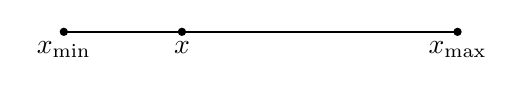
\begin{tikzpicture}
\draw[thick] (0,0) -- (5,0);
  \fill (0,0) circle (1.5 pt); 
  \fill (1.5,0) circle (1.5 pt);
  \fill (5,0) circle (1.5 pt); 
\node[below] at (0,0) {$x_{\min}$};
\node[below] at (1.5,0) {$x$};
\node[below] at (5,0) {$x_{\max}$};
\end{tikzpicture}


\centering
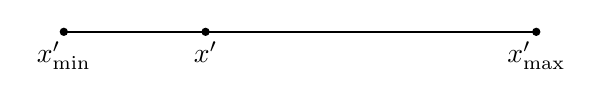
\begin{tikzpicture}
\draw[thick] (0,0) -- (6,0);
  \fill (0,0) circle (1.5 pt); 
  \fill (1.8,0) circle (1.5 pt);
  \fill (6,0) circle (1.5 pt); 
\node[below] at (0,0) {$x'_{\min}$};
\node[below] at (1.8,0) {$x'$};
\node[below] at (6,0) {$x'_{\max}$};
\end{tikzpicture}

\caption{Mapping x coordinates}
\label{fig:viewport-xform-x}
\end{figure}
In the figure ~\ref{fig:viewport-xform-x}, there is only one unknown, i.e., $x'$.
$x_{\min}$ to $x_{\max}$ is the region of the NDC and $x'_{\min}$ to $x'_{\max}$ is the region of screen coordinates. We want to find the expression for the point $x'$. The ranges are
\begin{align*}
x_{range} &= x_{\max} - x_{\min} \\ x'_{range} &= x'_{\max} - x'_{\min} 
\end{align*}
By the law of proportions $x$ and $x'$ are related by the following equation.
\begin{align*}
\frac{x-x_{\min}}{x_{range}} &= \frac{x'-x'_{\min}}{x'_{range}} 
\end{align*}
Simplifying this and solving for $x'$, we get 
\begin{align*}
x' &= x'_{\min} + (x-x_{\min}) \cdot \frac{x'_{range}}{x_{range}}
\end{align*}
We know the maximum interval of x coordinates for ndc and screen coordinates.
\begin{align*}
ndc_{interval} &= [-1,+1] \\
screen_{interval} &= [v_x,v_x+width] \\
x_{range} = +1 - -1 &= 2 \\
x'_{range} = v_x+width - v_x &=  width \\
x_{\min} &= -1 \\
x'_{\min} &= v_x
\end{align*}
Putting this in the solution for $x'$ we obtained earlier, we get
\begin{align*}
x' &= v_x + (x + 1) \cdot \frac{\text{width}}{2} \\
  x' &= v_x + \frac{\text{width}}{2} + x \cdot \frac{\text{width}}{2} \\
\end{align*}
\begin{equation}
    x' = x \cdot \frac{\text{width}}{2} + v_x + \frac{\text{width}}{2} 
\end{equation}

\subsection{Transforming Y Coordinates}
\begin{figure}[h]
\centering
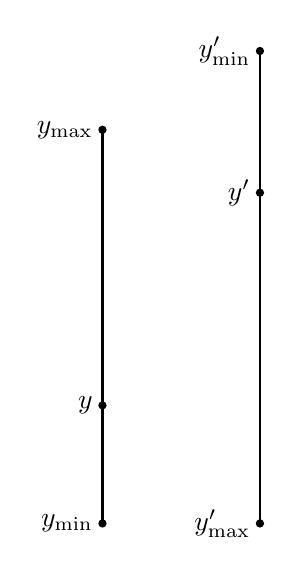
\begin{tikzpicture}
\draw[thick] (0,0) -- (0,5);
\draw[thick] (2,0) -- (2,6);
  \fill (0,0) circle (1.5 pt); 
  \fill (0,1.5) circle (1.5 pt);
  \fill (0,5) circle (1.5 pt); 
  \fill (2,0) circle (1.5 pt); 
  \fill (2,4.2) circle (1.5 pt);
  \fill (2,6) circle (1.5 pt); 

\node[left] at (0,0) {$y_{\min}$};
\node[left] at (0,1.5) {$y$};
\node[left] at (0,5) {$y_{\max}$};

\node[left] at (2,0) {$y'_{\max}$};
\node[left] at (2,4.2) {$y'$};
\node[left] at (2,6) {$y'_{\min}$};
\end{tikzpicture}
\caption{Mapping of y coordinates}
\label{fig:viewport-xform-y}
\end{figure}
As shown in the figure ~\ref{fig:viewport-xform-y}, our screen $y$-axis is inverted. We have the mappings $y_{\min} \rightarrow y'_{\max}$ and $y_{\max} \rightarrow y'_{\min}$.  
Therefore, by the law of proportions, $y$ and $y'$ are related by the following equation:
\begin{align*}
\frac{y-y_{\min}}{y_{\max}-y_{\min}} &= \frac{y'_{\max}-y'}{y'_{\max}-y'_{\min}}
\end{align*}
The above equation can be written as 
\begin{align*}
\frac{y-y_{\min}}{y_{range}} &= \frac{y'_{\max}-y'}{y'_{range}}
\end{align*}
Simplifying this, and solving for y' we get 
\begin{align*}
y' = y'_{max}-(y-y_{\min})\cdot \frac{y'_{range}}{y_{range}}
\end{align*}
We know the maximum interval of y coordinates for ndc and screen coordinates.
\begin{align*}
ndc_{interval} &= [-1,+1] \\
screen_{interval} &= [v_y,v_y+height] \\
y_{range} = +1 - -1 &= 2 \\
y'_{range} = v_y+height - v_y &=  height \\
y_{\min} &= -1 \\
y'_{\min} &= v_y
\end{align*}
Putting this in the solution for $y'$ we obtained earlier, we get
\begin{align*}
y' &= v_y + height - (y + 1) \cdot \frac{\text{height}}{2} \\
  y' &= v_y + height - \frac{\text{height}}{2} - y \cdot \frac{\text{height}}{2} \\
  y' &= v_y + \frac{\text{height}}{2} - y \cdot \frac{\text{height}}{2} \\
\end{align*}
\begin{equation}
y' = - y \cdot \frac{\text{height}}{2} + v_y + \frac{\text{height}}{2} \\    
\end{equation}
\subsection{Transforming Z Coordinates}

We need to transform NDC coordinates to depth in the interval \([0,\text{depth}_{\max}]\).  
We can find the expression for transformation as:

\begin{align*}
z' &= z'_{\min} + (z - z_{\min}) \cdot \frac{z'_{\text{range}}}{z_{\text{range}}}
\end{align*}

Putting the known values we get:

\begin{align*}
z' &= 0 + (z + 1) \cdot \frac{\text{depth}_{\max}}{2} \\
\end{align*}
\begin{equation}
       z' = z \cdot \frac{\text{depth}_{\max}}{2} + \frac{\text{depth}_{\max}}{2}
\end{equation}
\subsection{Deriving Viewport Matrix}
Using the results we obtained so far in this section, we can write the transformation equation as:
\[
\begin{bmatrix}
a_{00} & a_{01} & a_{02} & a_{03} \\
a_{10} & a_{11} & a_{12} & a_{13} \\
a_{20} & a_{21} & a_{22} & a_{23} \\
a_{30} & a_{31} & a_{32} & a_{33}
\end{bmatrix}
\cdot
\begin{bmatrix}
x \\
y \\
z \\
1
\end{bmatrix}
=
\begin{bmatrix}
x \cdot \frac{\text{width}}{2} + v_x + \frac{\text{width}}{2}  \\
- y \cdot \frac{\text{height}}{2} + v_y + \frac{\text{height}}{2} \\
z \cdot \frac{\text{depth}_{\max}}{2} + \frac{\text{depth}_{\max}}{2} \\
1
\end{bmatrix}
\]
By the deduction technique used in the previous sections, we can find the required matrix as:
\begin{equation}
\begin{bmatrix}
\frac{\text{width}}{2} & 0 & 0 & v_x + \frac{\text{width}}{2} \\
0 & -\frac{\text{height}}{2} & 0 & v_y + \frac{\text{height}}{2} \\
0 & 0 & \frac{\text{depth}_{\max}}{2} & \frac{\text{depth}_{\max}}{2} \\
0 & 0 & 0 & 1
\end{bmatrix}
\end{equation}
\section{Hidden Surface Removal}
To render objects convincingly and to optimize the process, we use depth buffering and back face culling. If depth buffering is not used, we always have to render objects starting from distant objects to the near objects. This will introduce sorting overhead, and even with sorting of triangles some types of objects can't be rendered convincingly. If backface culling is not used, we always have to rasterize triangles we won't see anyway, thus adding the overhead.
\subsection{Backface Culling}
By not rendering faces that we don't see we can save processor cycles.
After converting a triangle to screen space, we calculate its signed area and check if it is less than or equal to zero \footnote{area = 0 means, the triangle is made up of collinear points}. If it is so, the triangle is not rendered. This is valid because when we make the mesh, we specify vertices of each triangle in counter-clockwise order.And the triangles facing away from us will have signed area less than zero.
\subsection{Depth Buffering}
In addition to screen pixels, we store depth information for each pixel.
We draw a pixel only if the pixel's depth is less than the stored depth for that pixel. We do two kinds of depth buffering with respect to two kinds of camera we have. When the scene is rendered with perspective cameara, we use inverse w-buffering and when the scene is rendered with orthographic camera, we use normal z-buffering.
We get w from clip-space vertex, and we get z from screen-space vertex. 

\section{3D Scene}
The 3D scene is a collection of descriptions of parameters for the camera, meshes, textures, lights, and geometric objects along with their initial modeling transforms. The hierarchical object relationship is out of scope for our book. We use a custom text format for the scene description, which is explained later. 

\section{Rendering Problems}
While making the renderers for the upcoming chapters, you might be facing many rendering problems like in the following list. We will describe how to solve each of them in the respective chapters.
\vspace{1em} 
\begin{enumerate}
	\item Empty screen
    \item Abrupt program termination 
    \item Inverted rendered images
    \item Jagged edges on triangles
    \item Texture distortions
    \item Far objects rendered in front of near objects
    \item Extra pixels on the boundary of triangles
    \item Incorrect lighting and shading
\end{enumerate}
\vspace{1em} 

\clearpage